\documentclass[11pt, oneside]{article}   	% use "amsart" instead of "article" for AMSLaTeX format
\usepackage{geometry}                		% See geometry.pdf to learn the layout options. There are lots.
\geometry{letterpaper}                   		% ... or a4paper or a5paper or ... 
%\geometry{landscape}                		% Activate for for rotated page geometry
%\usepackage[parfill]{parskip}    		% Activate to begin paragraphs with an empty line rather than an indent
\usepackage{graphicx}				% Use pdf, png, jpg, or eps� with pdflatex; use eps in DVI mode
								% TeX will automatically convert eps --> pdf in pdflatex		
\usepackage{amssymb}
\usepackage{amsmath}
\usepackage{parskip}
\usepackage{color}
\usepackage{hyperref}

\title{Orthogonality of sine and cosine:  Paul}
%\author{The Author}
%\section{}
%\subsection*{}
\date{}							% Activate to display a given date or no date

\graphicspath{{/Users/telliott_admin/Dropbox/Tex/png/}}
% \begin{center} 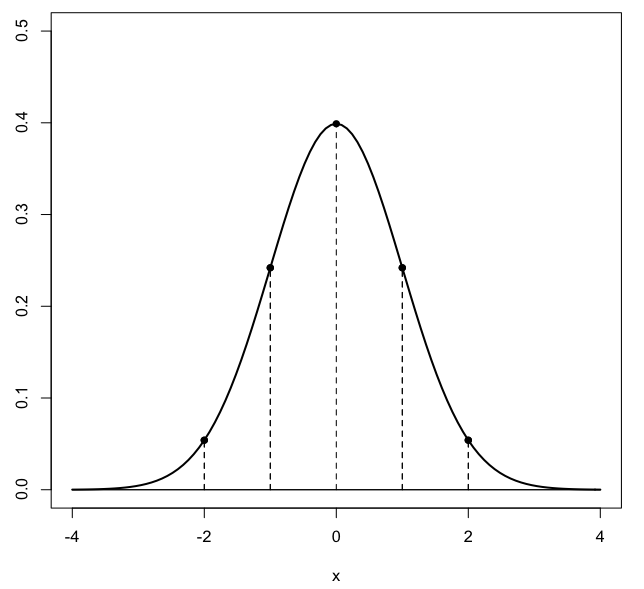
\includegraphics [scale=0.4] {gauss3.png} \end{center}
\begin{document}
\maketitle
\Large
We're going to look at integrals of products of trig functions.  We're going to show that certain products are orthogonal, the integrals are zero except for self times self.  The development comes from Paul's lectures on Differential Equations. 

To begin with, we recall our trig identities:

\[\cos s + t = \cos s \cos t - \sin s \sin t \]
\[\cos s - t = \cos s \cos t + \sin s \sin t \]
\[\sin s + t = \sin s \cos t + \sin t \cos s \]
\[\sin s - t = \sin s \cos t - \sin t \cos s \]
We add and subtract pairs of the above to obtain
\[\frac{1}{2} (\cos s + t  + \cos s - t) = \cos s \cos t  \]
\[\frac{1}{2} (\cos s - t  - \cos s + t) = \sin s \sin t  \]
\[\frac{1}{2} (\sin s + t  - \sin s - t) = \sin t \cos s  \]
\subsection*{cosine}
We're interested in the set of functions $\cos n \pi x /L$, for $n \in {1,2,3, \dots}$.  In general, we wish to evaluate
\[ \int_{-L}^{L} \cos \frac{n\pi x}{L} \cos \frac{m\pi x}{L} \ dx \] 
We note that cosine is an \emph{even} function, so 
\[ =  2\int_{0}^{L} \cos \frac{n\pi x}{L} \cos \frac{m\pi x}{L} \ dx \] 
We have three cases.  First $n=m=0$
\[ =  2\int_{0}^{L} \ dx = 2L\] 
Then, $n=m\ne0$
\[ =  2\int_{0}^{L} \cos^2 \frac{n\pi x}{L} \ dx \] 
From above
\[\frac{1}{2} (\cos s + t  + \cos s - t) = \cos s \cos t  \]
For $s=t$
\[\frac{1}{2} (\cos 2s  + 1) = \cos^2 s   \]
So the integral is
\[ =  \int_{0}^{L} 1 + \cos \frac{2n\pi x}{L}  \ dx \] 
\[ = x + \frac{L}{2n\pi}  \sin \frac{2n\pi x}{L} \bigg |_0^L \]
\[ = L + \frac{L}{2n\pi}  \sin 2n\pi = L \]
since $n$ is an integer.  The third case is $n \ne m$ and neither is zero.
\[ 2\int_{0}^{L} \cos \frac{n\pi x}{L} \cos \frac{m\pi x}{L} \ dx \] 
\[ = \int_{0}^{L} \cos \frac{n\pi x}{L} + \frac{m\pi x}{L} + \cos \frac{n\pi x}{L} - \frac{m\pi x}{L} \ dx \]
\[ = \int_{0}^{L} \cos \frac{(n+m)\pi x}{L} + \cos \frac{(n-m)\pi x}{L}  \ dx \]
\[ = \frac{L}{(n+m)\pi} \sin \frac{(n+m)\pi x}{L} + \frac{L}{(n-m)\pi} \sin \frac{(n-m)\pi x}{L}  \bigg |_0^L \] 
But since $n$ and $m$ are integers, both sine terms are zero.
\subsection*{sine}
Our next set of functions involve
\[ \int_{-L}^{L} \sin \frac{n\pi x}{L} \sin \frac{m\pi x}{L} \ dx \] 
This is the product of two odd functions, which is an even function!  So again, we can change the limits:
\[ 2 \int_{0}^{L} \sin \frac{n\pi x}{L} \sin \frac{m\pi x}{L} \ dx \] 
Next, if $m=n$ we will not them be equal to zero.  So we start our analysis with $n=m\ge1$
\[ 2 \int_{0}^{L} \sin^2 \frac{n\pi x}{L}  \ dx \] 
\[ = \int_{0}^{L} 1 - \cos  \frac{2n\pi x}{L}  \ dx \]
\[ = x - \frac{L}{2n\pi } \sin \frac{2n\pi x}{L}  \bigg |_0^L \] 
\[ = L - \frac{L}{2n\pi } \sin 2n\pi  \] 
but since $n$ is an integer the second term is zero so the integral is just $L$.  Last we have
\[ 2 \int_{0}^{L} \sin \frac{n\pi x}{L}  \sin \frac{m\pi x}{L} \ dx \] 
Going back to our identities we get
\[ = \int_{0}^{L} \cos \frac{(n-m)\pi x}{L} -  \cos \frac{(n+m) \pi x}{L} \ dx \] 
\[ = \frac{L}{(n-m)\pi} \sin \frac{(n-m)\pi x}{L} -  \frac{L}{(n+m)\pi} \sin \frac{(n+m) \pi x}{L}  \ \bigg |_0^L \] 
\[ = \frac{L}{(n-m)\pi} \sin (n-m)\pi -  \frac{L}{(n+m)\pi} \sin (n+m) \pi  \]
\[ = 0 \]
\subsection*{sine and cosine}
The interval here cannot be $0 \rightarrow L$, because the integral will actually be non-zero.  Instead we do 
\[ \int_{-L}^{L} \sin \frac{n\pi x}{L} \cos \frac{m\pi x}{L} \ dx \] 
but the product of an even function and an odd function is an odd function so this integral is zero.

Let me include Paul's figures summarizing what we have so far.
\begin{center} 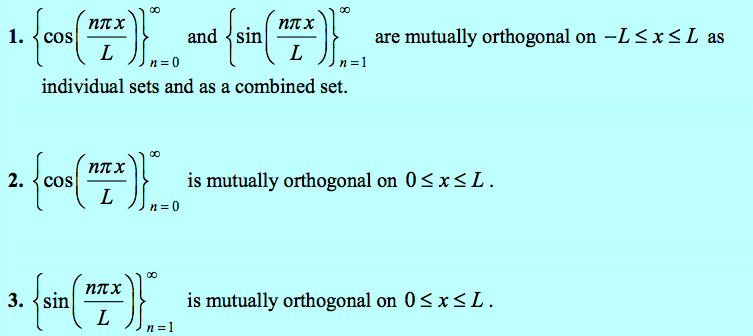
\includegraphics [scale=0.5] {Paul_ortho1.png} \end{center}
\begin{center} 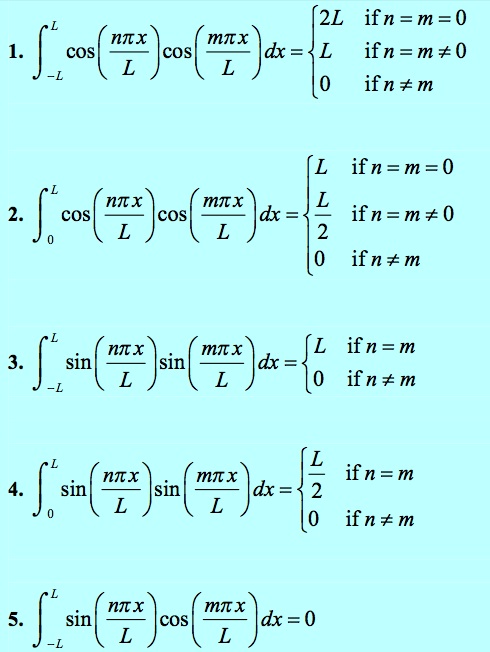
\includegraphics [scale=0.5] {Paul_ortho2.png} \end{center}


\end{document}  